 \documentclass[11pt]{article}
% \pagestyle{empty}
\usepackage{mathtools}
\DeclarePairedDelimiter\ceil{\lceil}{\rceil}
\DeclarePairedDelimiter\floor{\lfloor}{\rfloor}
\usepackage{algorithmicx}
\usepackage{algpseudocode}
\usepackage{algorithm}
\usepackage[makeroom]{cancel}

\usepackage[letterpaper, portrait, margin=1in]{geometry}
\usepackage{epsf}
\usepackage{pseudocode}
% \usepackage{times}
% \usepackage{mathptm}

\def\O{\mathop{\smash{O}}\nolimits}
\def\o{\mathop{\smash{o}}\nolimits}
\newcommand{\e}{{\rm e}}
\newcommand{\R}{{\bf R}}
\newcommand{\Z}{{\bf Z}}

\title{CS 124, Problem Set 6}
\author{Jessica Wang}
\date{April 8, 2016}

\begin{document}
\maketitle
\section*{Problem 1}
The partially reflecting boundry can be represented given some number of spots $n$, the expected amount of steps is takes to get from spot $i$ to spot $n$ can be represented by the recurrence relation $T(i)$ where $T(0)= \frac{1}{2}T(0) + \frac{1}{2}T(1) + 1$, $T(n)=0$ and $T(i) = \frac{1}{2}T(i-1) + \frac{1}{2}T(i+1) +1$. Solving this recurrence relation $T(i)$ will give the expected number of steps. I solved this recurrence by finding $T(i)$ the smaller values of $n$ as follows:

\begin{align*}
n &= 0\\
T(0) &= 0\\ 
\end{align*}
\begin{align*}
n &= 1\\
T(1) &= 0 \\
T(0) &= \frac{1}{2} T(0) + 1 \\
\frac{1}{2}T(0) &= 1\\
T(0) &= 2\\ 
\end{align*}
\begin{align*}
n &=2 \\
T(2) &= 0 \\
T(1) &= \frac{1}{2} T(0) +1 \\
T(0) &= \frac{1}{2}T(0) + \frac{1}{2}(\frac{1}{2} T(0) +1) + 1 \\
\frac{1}{4}T(0) &=  \frac{3}{2} \\
T(0) &= 6 \\
T(1) &= 4 \\
\end{align*}
\begin{align*}
n &= 3 \\
T(3) &=  0\\
T(2) &=  \frac{1}{2}T(1) + 1\\
T(1) &=  \frac{1}{2}T(0) +  \frac{1}{2}(\frac{1}{2}T(1) + 1) +1 \\
\frac{3}{4}T(1) &= \frac{1}{2}T(0) + \frac{3}{2} \\
T(1) &= \frac{2}{3} T(0) + 2\\
T(0) &= \frac{1}{2}T(0) + \frac{1}{2}(\frac{2}{3} T(0) + 2) + 1\\
\frac{1}{6} T(0) &= 2 \\
T(0) &= 12\\
T(1) &= 10\\
T(2) &= 6\\
\end{align*}
Extrapolating from this you find the expected number of steps to reach spot $n$ by starting at spot $i$ is $T(i) = (n-i)(n+i+1)$
\section*{Problem 2}
The Ford Fulkerson Algorithm was conducted using the following augmenting paths of the residual network (augmenting path shown in blue at each step)\\

Augmenting Path 1: Path has flow 3 with overall graph flow of 3\\
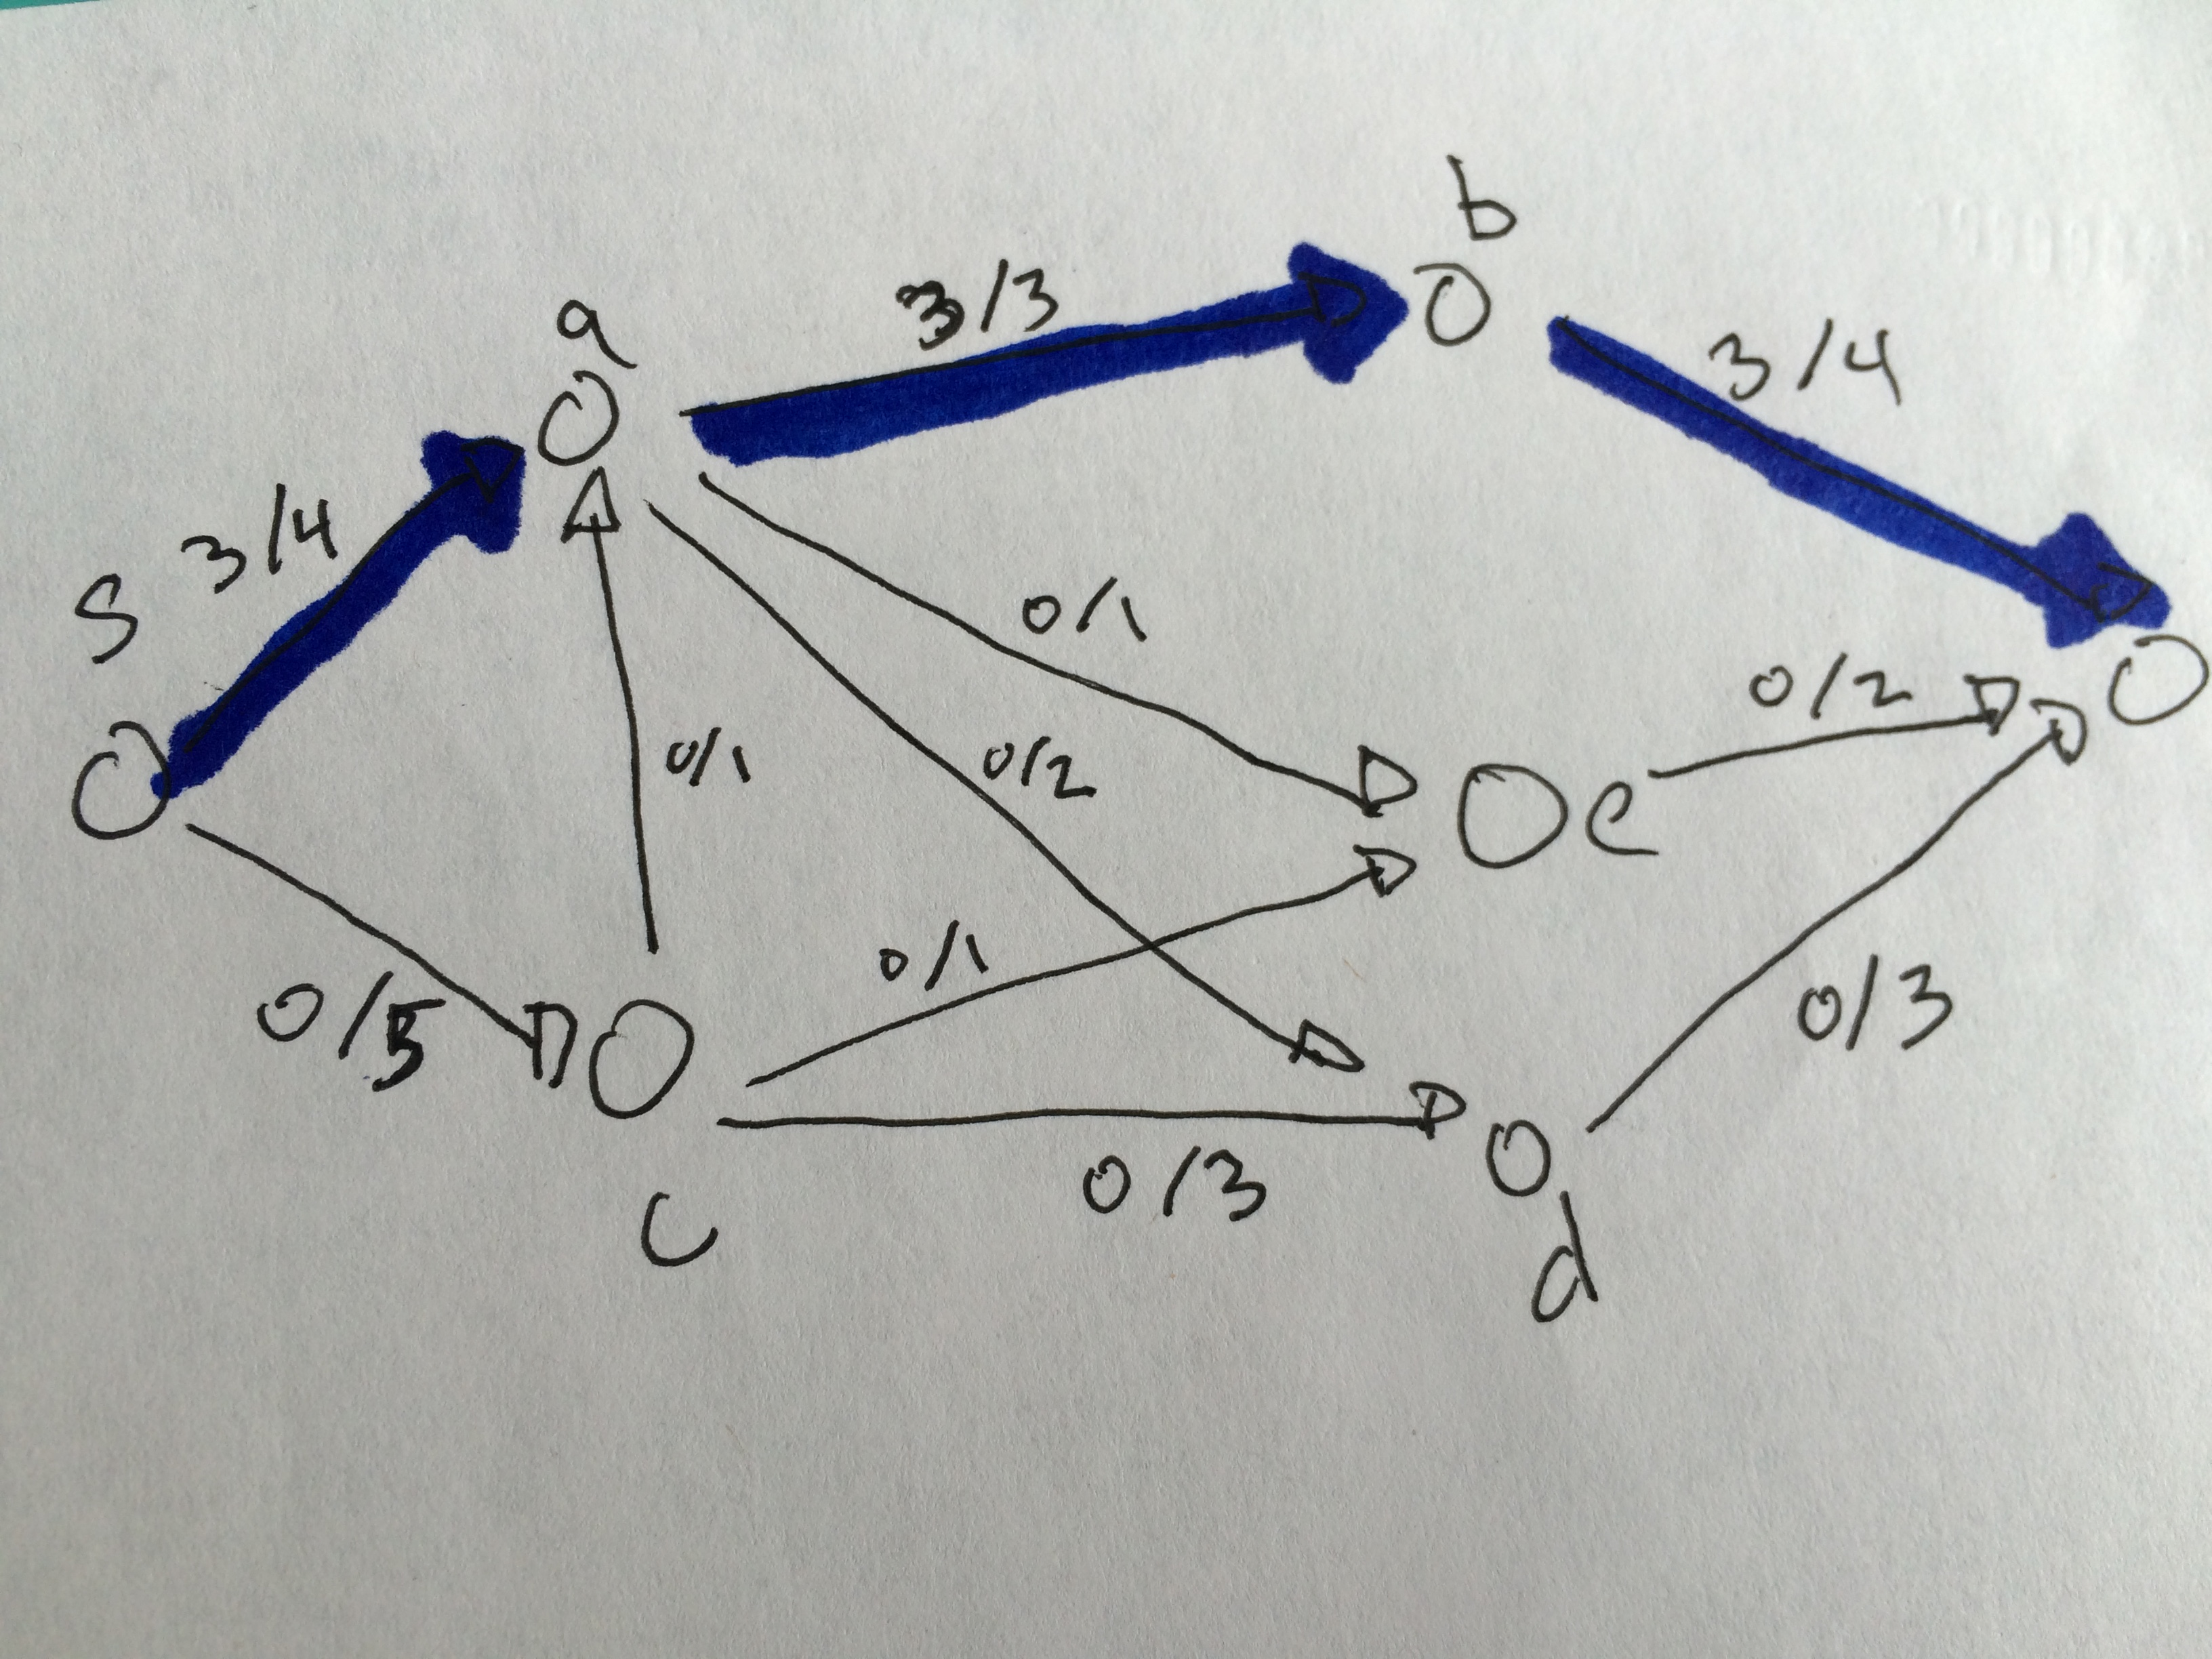
\includegraphics[scale=.1]{IMG_5551.jpg} \\

Augmenting Path 2: Path has flow 3 with overall graph flow of 6\\
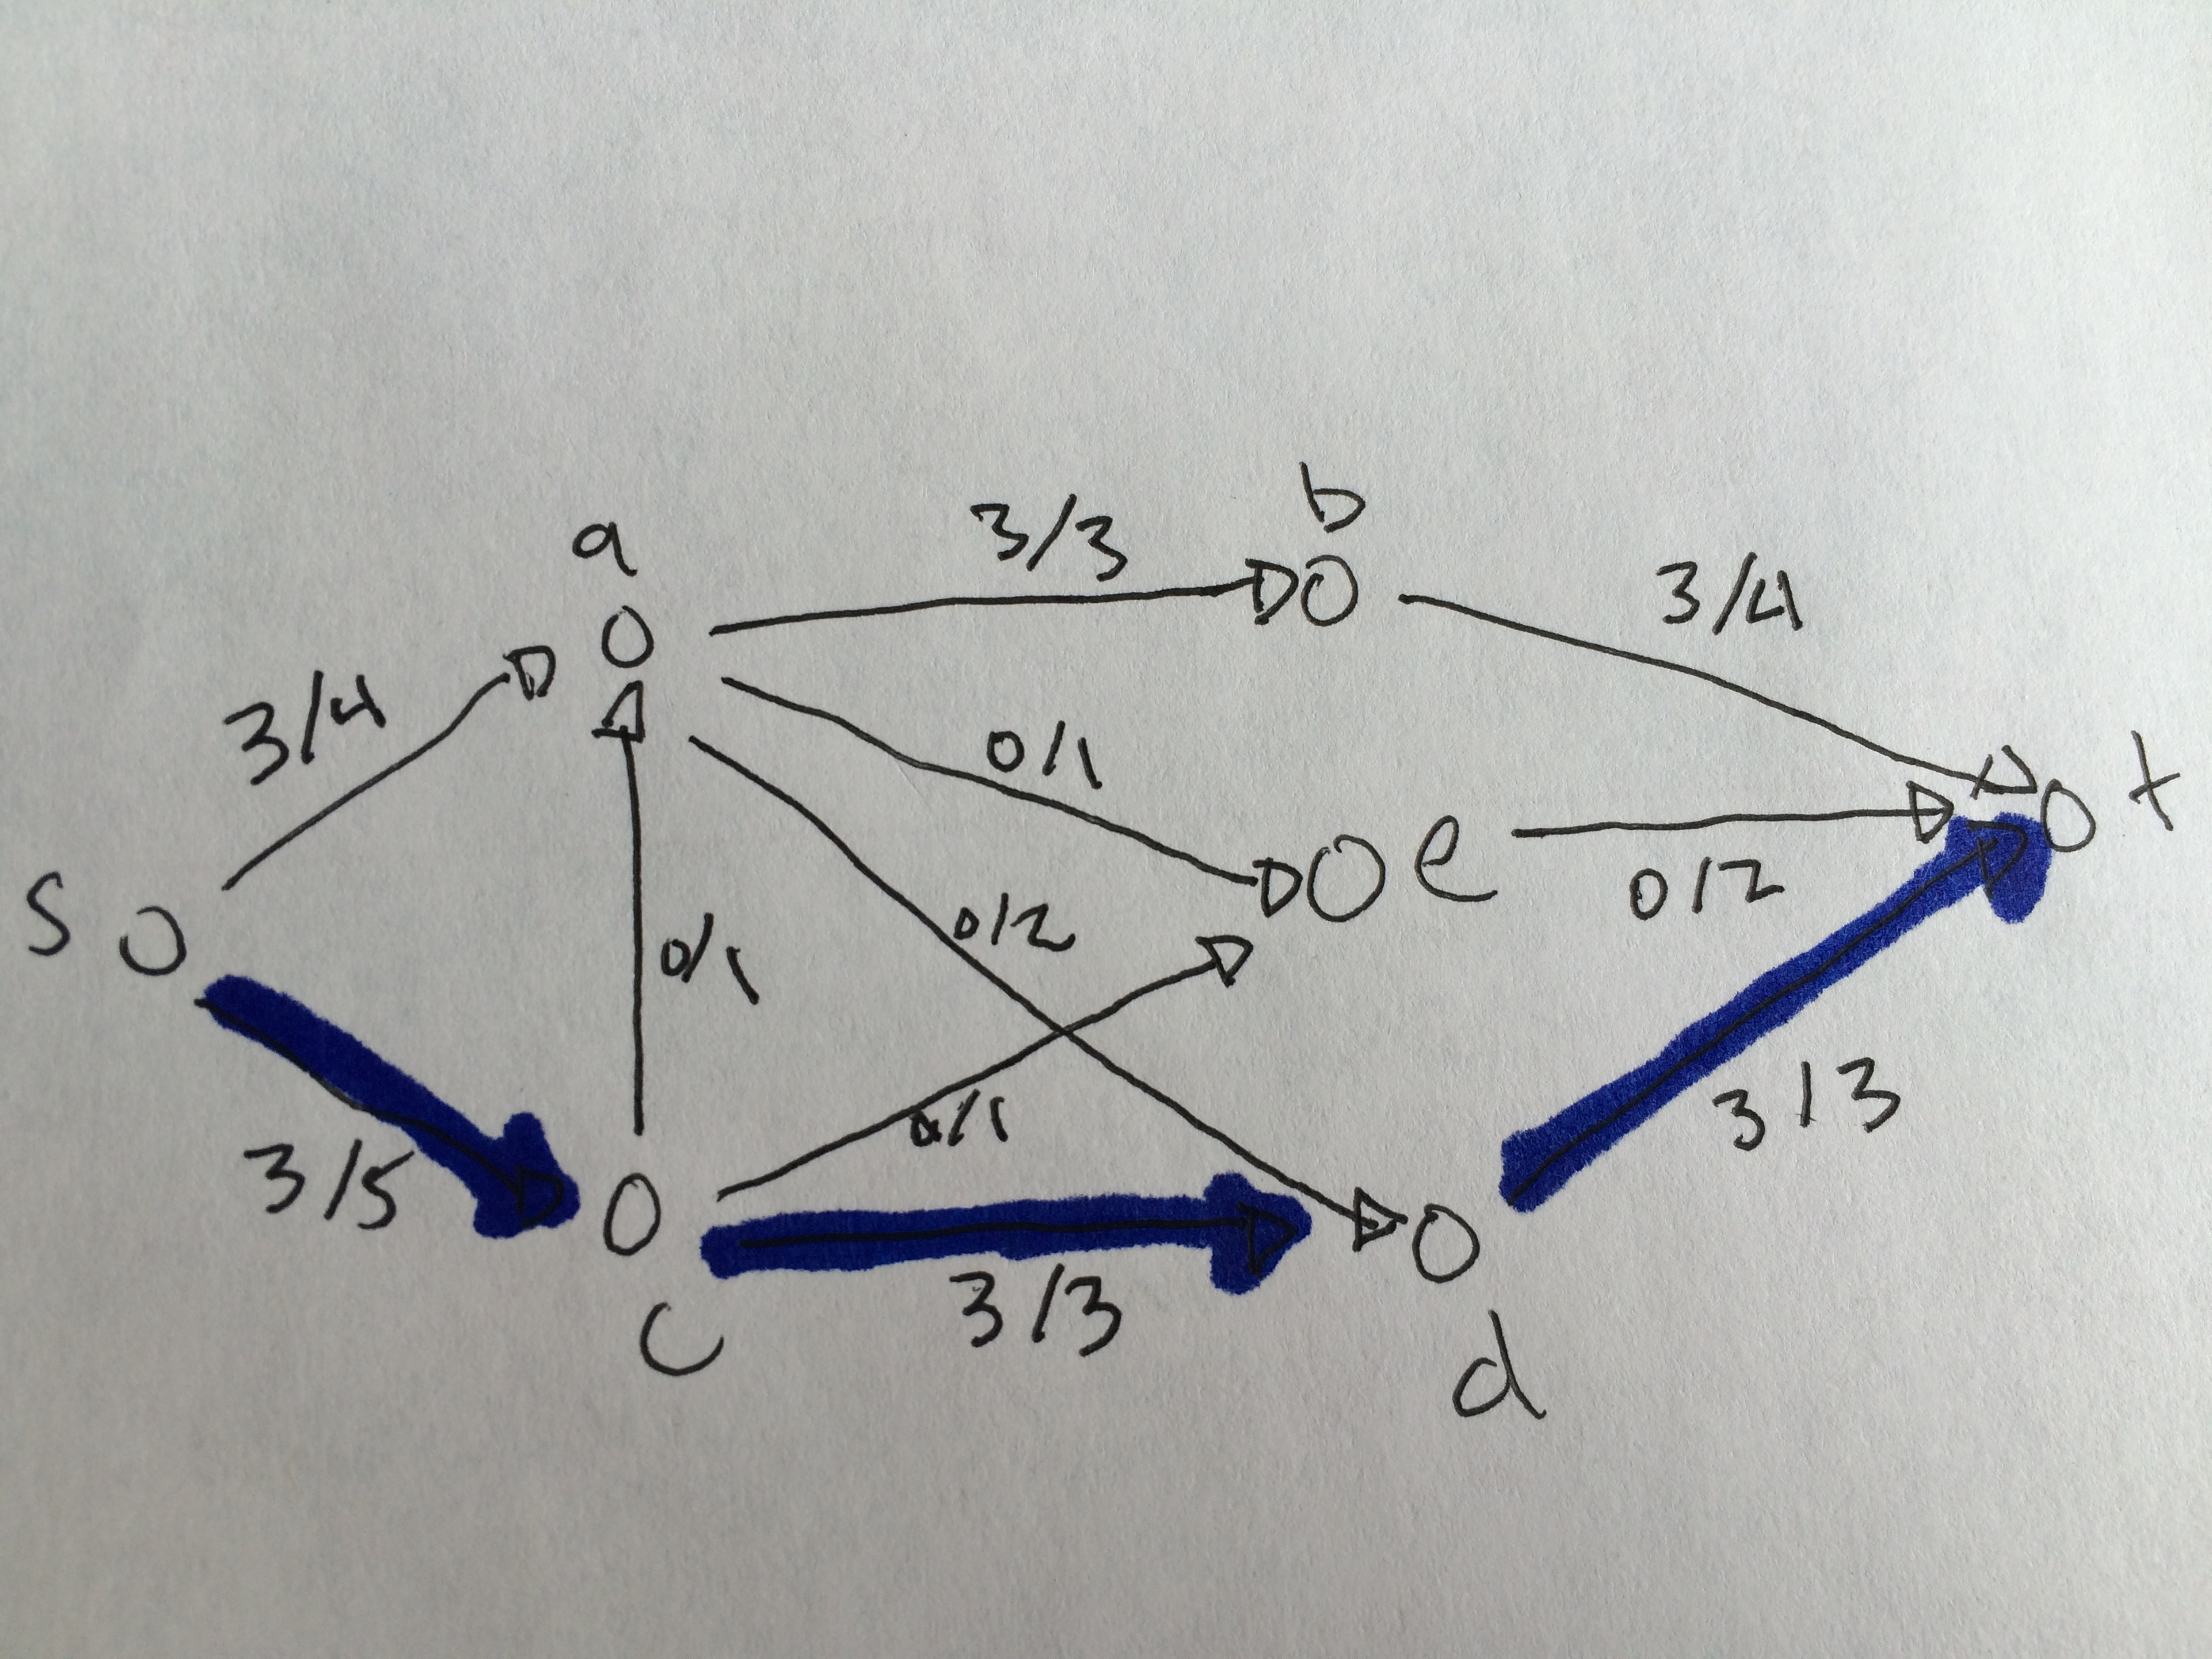
\includegraphics[scale=.1]{IMG_5552.jpg} \\

Augmenting Path 3: Path has flow 1 with overall graph flow of 7\\
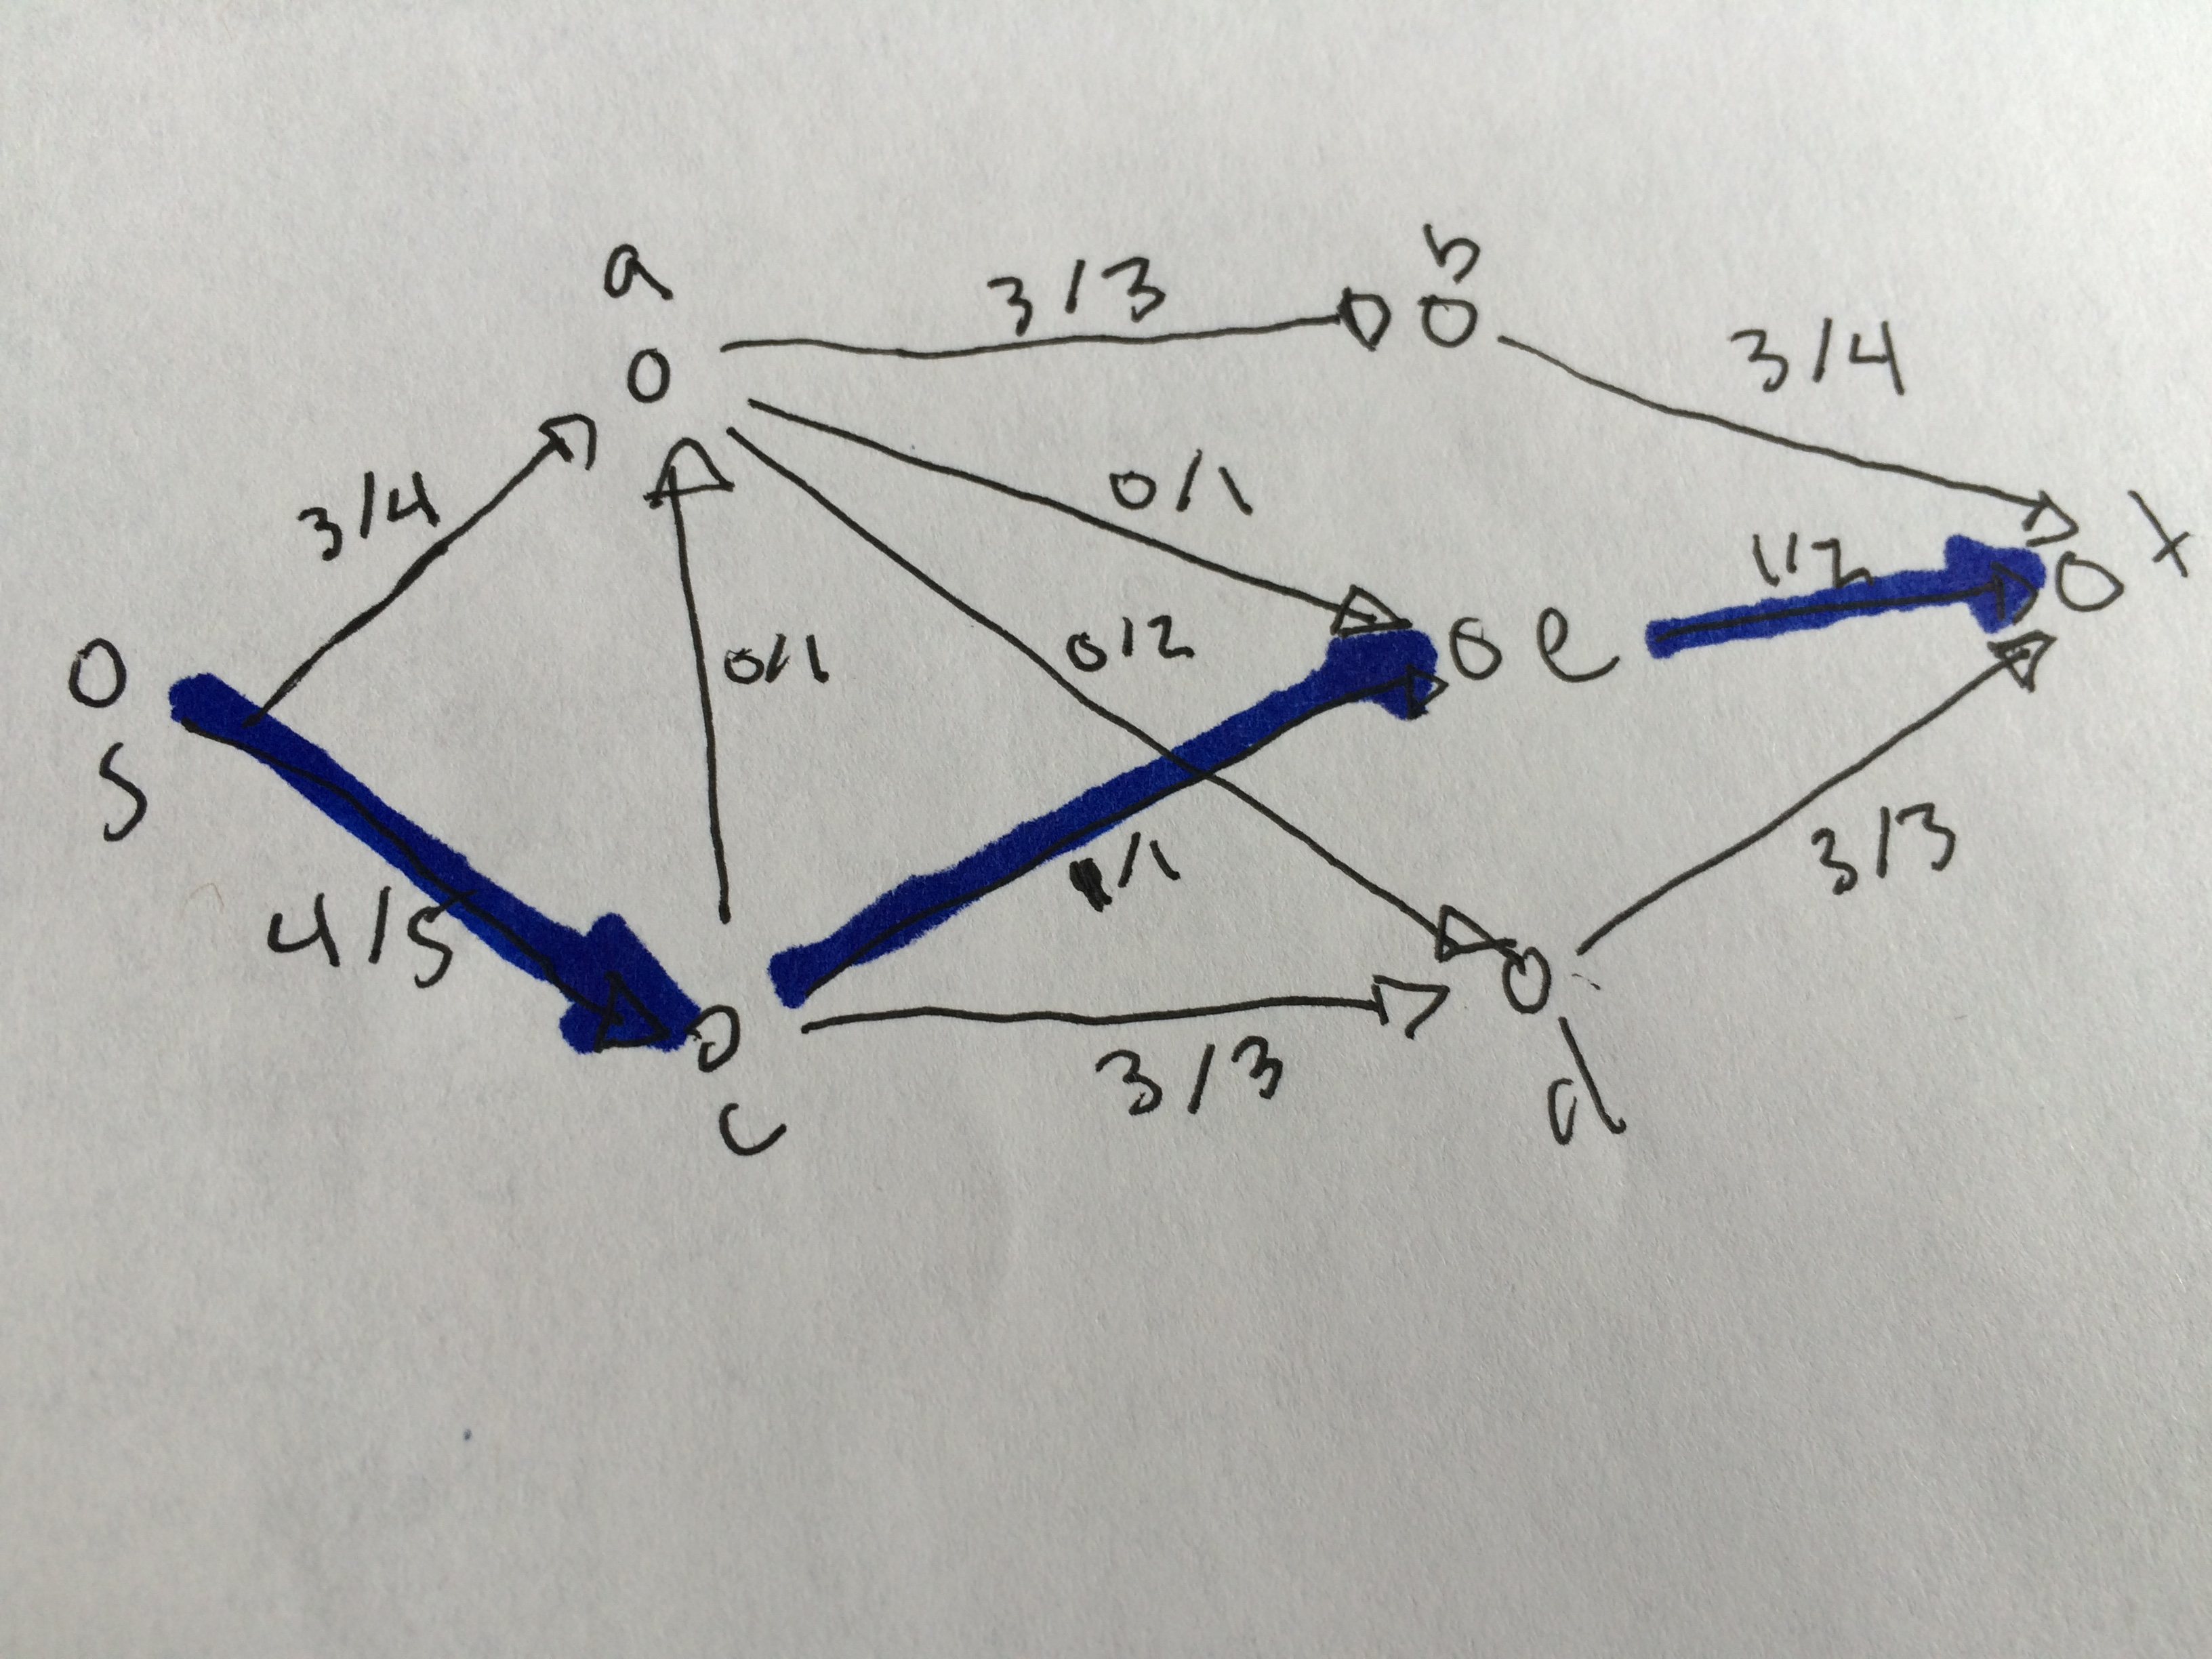
\includegraphics[scale=.1]{IMG_5553.jpg} \\

Augmenting Path 4: Path has flow 1 with overall graph flow of 8\\
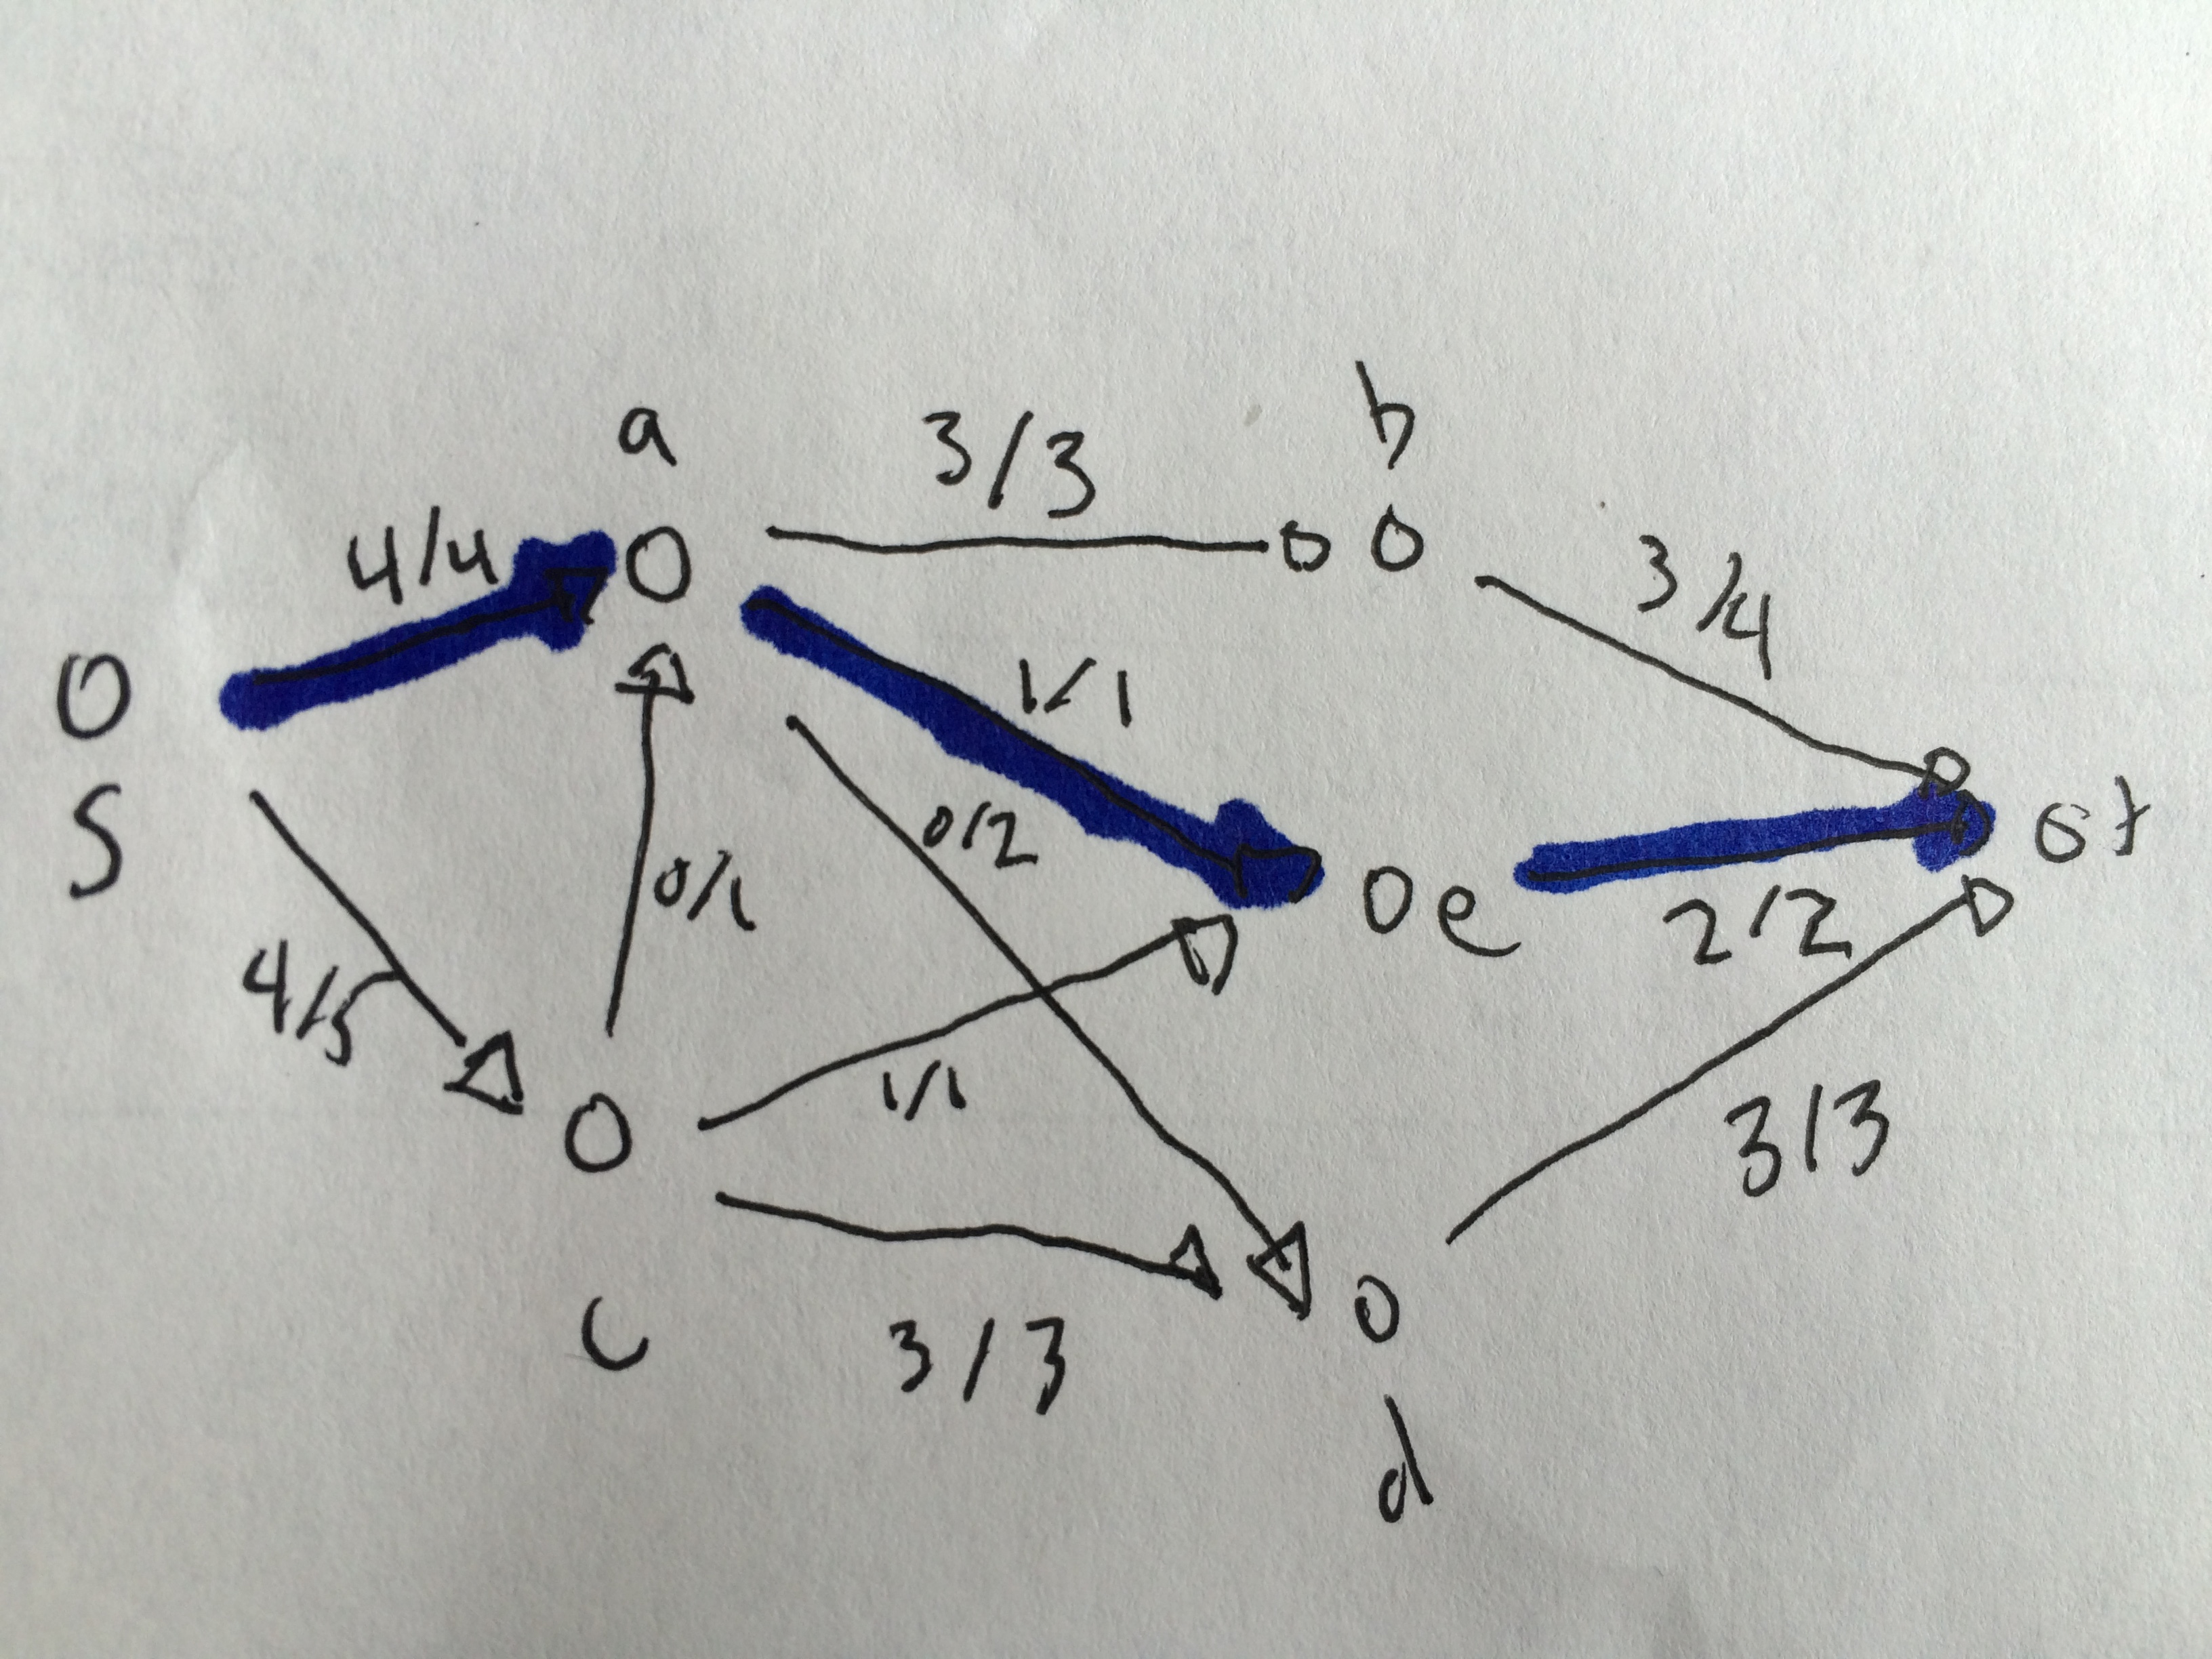
\includegraphics[scale=.1]{IMG_5554.jpg} \\

The final graph with the flow values of each edge the final overall flow value of 8 is shown below. The edges of the cut are indicated by the dashed edges. This was found by running a DFS from the sink and marking which vertices are reachable $(s,a,c,d)$ and which vertices are unreachable $(b,e,t)$. The edges between these two groups are where the cuts would be made. The final cut value is also 8.\\
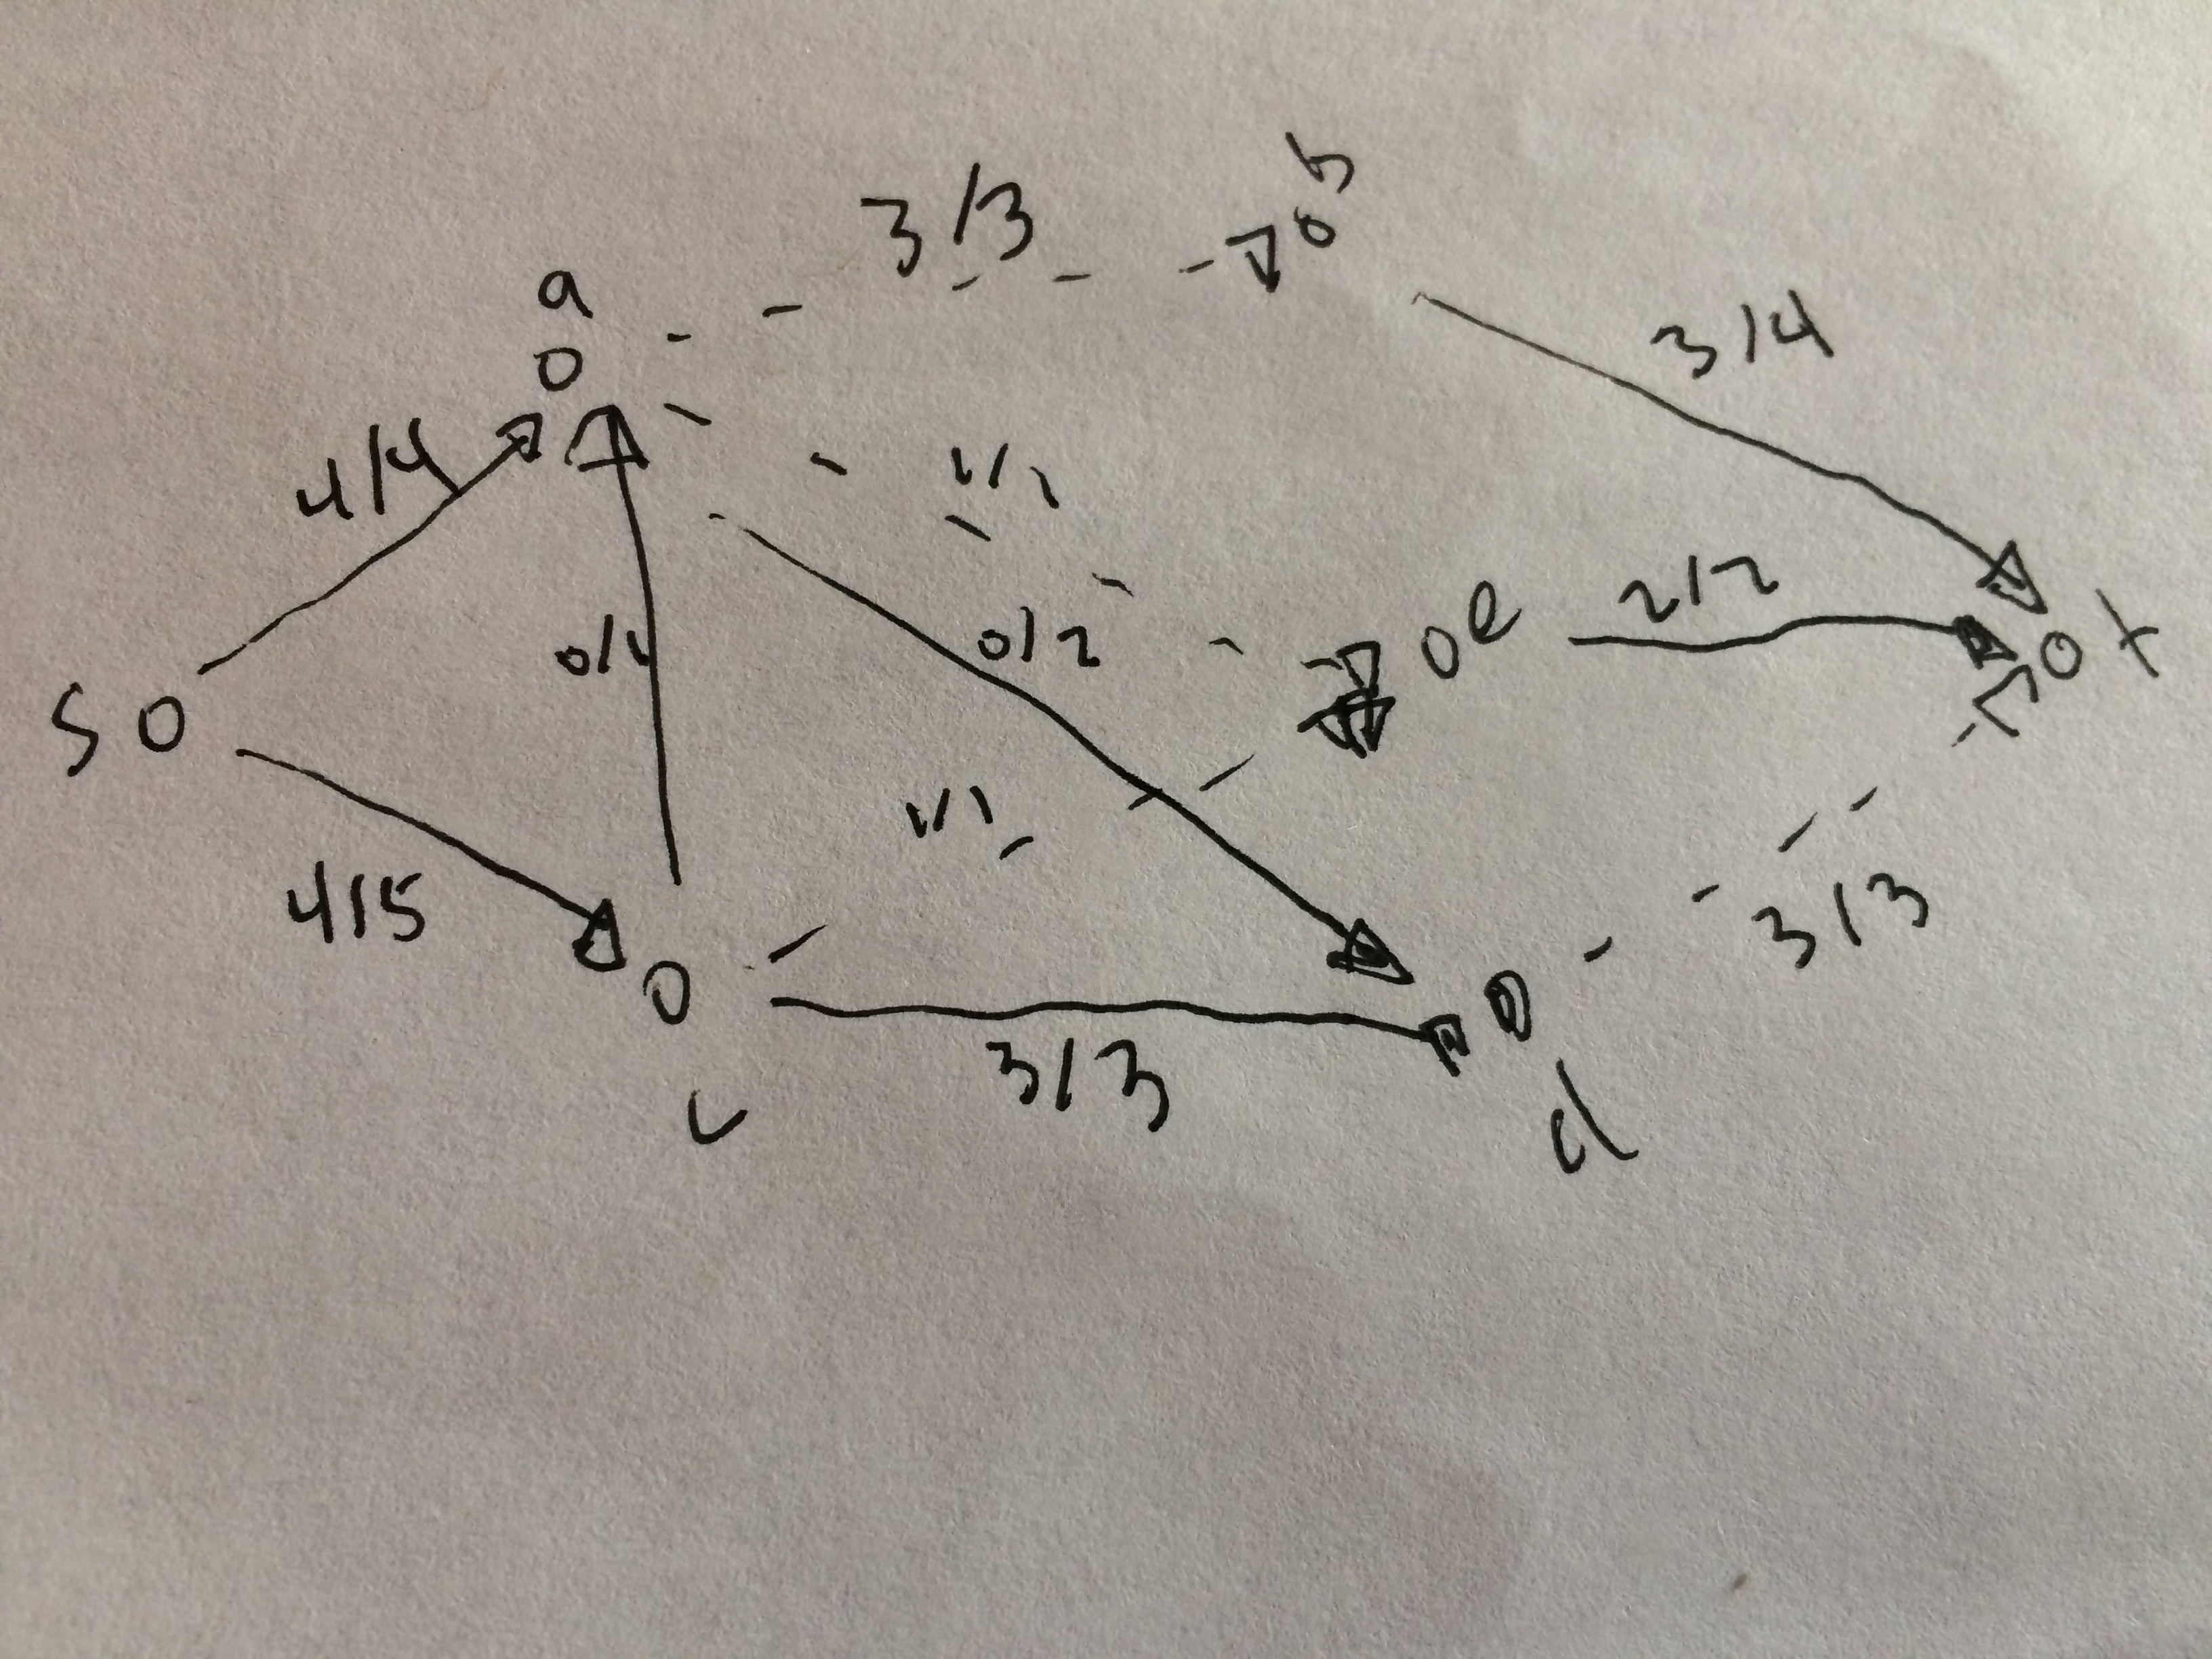
\includegraphics[scale=.1]{IMG_5556.jpg} \\
\section*{Problem 3}
\subsection*{Part 1}
We can generalize this problem to the general maximum flow problem by slightly changing the graph. Let $S_1, S_2, ..., S_x$ be the multiple sources of the original graph and $T_1, T_2, ..., T_y$ be the multiple sinks of the original graph. Add a new source $S'$ which has a directed edge towards all sources $S_i$ with infinite capacity for flow, thus changing each $S_i$ away from being a source to being a normal vertex. Similarly add a new sink $T'$ which each $T_i$ has a directed edge towards $T'$ with inifinite capacity for flow, thus changing each $T_i$ away from being a sink to being a normal vertex. This would be similar to the matching, bipartite question discuessed in class. This converted graph now has a single source and sink, which allows the Ford Fulkerson modified DFS to carry on as usually when parsing through the graph. Adding this new source and sink does not change the maximum flow of the graph because since the edges connect to these points have infinite capacity, allowing none of these edges to be the bottle neck of the flow. Since any amount of flow can go into $S_i$ and the constricting factor of $S_i$ is the capacity on the edges coming out of $S_i$. It is similar to the sinks $T_i$ could have infinite flow out and are bottlenecked by the capacity of the edges going into $T_i$. Thus the new source and sink allow infinite capacity into each $S_i$ with the same capacities out and inifinite capacity out of each $T_i$  and the same capacities in, making the maximum flow of our converted graph to be the same as the maximum flow of the original graph. This algorithm would take the same run time as Ford Fulkerson and could be done with linear programing.

\subsection*{Part 2}
We can generalize this problem to the general maximum flow problem by slightly changing the graph. Let $v_1, v_2, ..., v_x$ be the verticies within the graph each of which have capacity $c_1, c_2, ...., c_x$ respectively. For each vertex $v_i$ let the edges into $v_i$ be $e_1, e_2, ..., e_y$ and the edges out of $v_i$ be $e'_1, e'_2, ..., e'_z$. For each vertex $v_i$ create an additional vertex $v'_i$ such that $e_1, e_2, ..., e_y$ direct to $v_i$, there is a single edge with capacity $c_i$ directed from $v_i$ to $v'_i$ and have $e'_1, e'_2, ..., e'_z$ directed out of $v'_i$. Thus essentially we are changing each vertex $v_i$ into to verticies $v_i$ and $v'_i$ which are connected between with an edge, $e''_i$ with capacity of $v_i$.  Neither $v_i$ or $v'_i$ would have a capacity anymore, allowing the converted graph to be in the standard form to be able to use Ford Fulkerson algorithm and solve the problem with linear programing. Creating this additional vertex and the edge between them allows us to represent the capacity of $v_i$ in the newley created edge. The edge will bottleneck for the flow going into the original $v_i$ when calculating the Ford Fulkerson algorithm when the graph has to transverse $e''i$ into $v'_i$. The edge will also bottle neck the flow going out of hte original $v_i$ when calculating the Ford Fulkerson algorithm when the graph has to traverse $e''_i$ out of $v_i$. In this way the additional vertex and edge are able to bottleneck the original vertex $v_i$ at capacity $c_i$ both in and out of the pair $v_i, v'_i$ which represents the original $v_i$. In this way the Ford Fulkerson algorithm will calculate the same maximum flow of the converted graph as the maximum flow of the original graph where the verticies had capacities.

\section*{Problem 4}
\subsection*{Part 1}
 To reduce this problem to an linear programing problem we define some maximizing function in this case and list the constraints necessary to generate the linear equations to solve the max flow problem given some conditions, which in this case is as the problem lists. Since we are trying to maximize flow, we define our maximizing function as:\\
\begin{align*}
max \bigg( \sum_{(u,v) \in E}^{} f(u,v) \bigg)
\end{align*}
subject to:
\begin{align*}
\text{Capacity Constraints: }&f(u,v) \leq c(u,v)\\
\end{align*}
However, for this specific problem, our conservation of flow changes:
\begin{align*}
\text{Flow Conservation: }&\frac{1}{2}\sum_{(u,v) \in E}^{} f(u,v) \leq \sum_{(u,v)\in E}^{} f(v,u) \\
u\not= s, v\not=t
\end{align*}
With a maximizing function with a generalize constraint, we have satisfied the conditions to convert a generalize flow graph with this particular characteristic (half flow out) into an LP problem. Thus since we know that linear programing problem can be solved in using a simplex as discussed in class, which runs in polynomial time.

\subsection*{Part 2}
To minimize the cost of the max flows we will run two linear programs. The first one will determine the max flow which can be generalized as:\\
\begin{align*}
max \bigg( \sum_{(u,v) \in E}^{} f(u,v) \bigg)
\end{align*}
subject to:
\begin{align*}
\text{Capacity Constraints: }&f(u,v) \leq c(u,v)\\
\text{Flow Conservation: }&\sum_{(u,v) \in E}^{} f(u,v) \leq \sum_{(u,v)\in E}^{} f(v,u) \\
u\not= s, v\not=t
\end{align*}

This will give us some max flow $d$, which we will use in the next linear program to determine min cost of the max flows:\\
\begin{align*}
minimize \bigg( \sum_{(u,v) \in E}^{} a(u,v)\times f(u,v) \bigg)
\end{align*}
where function $a(u,v)$ is the cost from vertex $u$ to $v$, subject to:\\
\begin{align*}
\text{Capacity Constraints: }&f(u,v) \leq c(u,v)\\
\text{Flow Conservation: }&\sum_{(u,v) \in E}^{} f(u,v) \leq \sum_{(u,v)\in E}^{} f(v,u) &
u\not= s, v\not=t\\
\text{Required Flow: }& \sum_{w \in V}^{} f(s,w) = d \\
&\sum_{w \in V}^{} f(w,t) = d
\end{align*}
where $s$ is the source and $t$ is the sink.\\
With a minimizing function with a generalize constraint, we have satisfied the conditions to convert a generalize flow graph with this particular characteristic (half flow out) into an linear programing problem. Thus since we know that the first linear programing problem can be solved in $O(m max |f|)$ with Ford-Fulkerson's algorithm and the second linear programing problem can be solved using a simplex as discussed in class, which runs in polynomial time.

\section*{Problem 5}
\subsection*{Increase Capacity}
When increasing flow of a given edge $e$ consider the state of $e$ before increasing the flow. Let $e$ be "saturated" if the flow through the edge is equivelent to the capacity of the edge. When increasing the capacity of $e$, the maximum flow of the graph will only change if $e$ was originally saturated. If $e$ started unsaturdated $e$ is not a bottleneck edge of the original graph and there must be some other edge $e'$ that is saturated and be a bottleneck for the maximum flow. If you increase the capacity for $e$, $e'$ will still be the bottleneck of the graph so no additional flow could go through with the original capacity and no additional flow could go through $e$ with the increased capacity. If $e$ in the original graph was saturated then $e$ could be the bottleneck of the original graph and preventing the maximum flow form increasing. Thus the maximum flow of the graph with the capacity of $e$ increased by one could be higher by one. To find if the new graph can increase in maximum flow, run a DFS on a residual network that has the amount of flow of the original graph at maximum flow but with the capacity of $e$ increased by one. Running the DFS starting at the source $S$, if we are able to reach the sink $T$ of the residual network, then it will indicate an augmenting path which will increase flow, similar to the Ford Fulkerson algorithm. If the path exists, it must go through $e$ because the original graph was already at maximum flow and no augmenting path would exist in the non-$e$ edges. If the DFS reaches $T$, then the maximum flow of the new graph would increase from the original maximum flow by 1. This algorithm would take the run time of DFS which is $O(|V|+|E|)$. 

\subsection*{Decrease Capacity}
Similar to increaseing capacity, the maximum flow if you decrease the capacity of $e$ will only change if $e$ was saturated in the original graph. If $e$ was unsaturated, there would be another edge $e'$ that is saturated and be the bottleneck edge of the graph which does not allow the maximum capacity to increase. By decreasing $e$ the original maximum flow could still flow through the graph so the maximum flow will not decrease. If $e$ is saturated it could be a bottleneck edge of the original graph, so decreasing the capacity of $e$ by one could lower the maximum flow by one. This would be because there was some augmented path from the Ford Fulkerson of the original graph that went through $e$ which increased the flow by one that the new graph can no longer have. To find this path, run two DFS algorithms. Let $e$ be from vertex $u$ to $v$. The first DFS would search for a path from $u$ to the source vertex $S$, which would be going against the direction of the edges. The second DFS would search for a path from $v$ to the sink vertex $T$. If both these DFS are successful then we have found an augmented path from $S$ to $T$ going through $e$. If this augmented path exists, it must be removed because $e$, which was originally saturated, has decreased in capacity by one. Thus if this path exists, the maximum flow will decrease by 1 and the flow through every edge in the path will decrease accordingly as well. This algorithm uses two DFS algorithms so the overall run time will be $O(|E|+|V|)$. 

\section*{Problem 6}
For the row player, the linear program can be represented by maximizing $z$ subject to $a+b+c+d = 1$, $-3a-6b+3c+7d+z \leq 0$, $-a+2b+2c-4d+z \leq 0$, $0a+2b-3c+5d+z \leq 0$ and $4a+0b+3c-7d+z \leq 0$. Using a linear programing solver online we found that the optimal situation was when $z = -.38422, a = .1509, b=.2762, c= .3791, d =.1938$. So the row player's strategy would be $(.1509, .2762, .3791, .1938)$ with .3842 payoff.\\
For the column player, the linear program can be represented by minimizing $z$ subject to $a+b+c+d = 1$, $-z+3a+b+0c-4d \leq 0$, $-z+6a-2b-2c+0d \leq 0$, $-z-3a+2b+3c-3d \leq 0$ and $-z-7a+4b-5c+7d \leq 0$. Using a linear programing solver online we found that the optimal situtation was when $z=-.3842, a=.1389, b=.2075, c=.4014, d=.2522$. So the column player's strategy is $(.1389, .2075, .4014, .2522)$ with a -,3842 payoff.\\
To make this game fair the column player should pay the row player $.38422$. 
\end{document}
